%\VignetteEngine{knitr::knitr}
%\VignetteIndexEntry{pbkrtest-introduction: Introduction to pbkrtest}
%\VignettePackage{pbkrtest}

\documentclass[11pt]{article}\usepackage[]{graphicx}\usepackage[]{xcolor}
% maxwidth is the original width if it is less than linewidth
% otherwise use linewidth (to make sure the graphics do not exceed the margin)
\makeatletter
\def\maxwidth{ %
  \ifdim\Gin@nat@width>\linewidth
    \linewidth
  \else
    \Gin@nat@width
  \fi
}
\makeatother

\definecolor{fgcolor}{rgb}{0.345, 0.345, 0.345}
\newcommand{\hlnum}[1]{\textcolor[rgb]{0.686,0.059,0.569}{#1}}%
\newcommand{\hlstr}[1]{\textcolor[rgb]{0.192,0.494,0.8}{#1}}%
\newcommand{\hlcom}[1]{\textcolor[rgb]{0.678,0.584,0.686}{\textit{#1}}}%
\newcommand{\hlopt}[1]{\textcolor[rgb]{0,0,0}{#1}}%
\newcommand{\hlstd}[1]{\textcolor[rgb]{0.345,0.345,0.345}{#1}}%
\newcommand{\hlkwa}[1]{\textcolor[rgb]{0.161,0.373,0.58}{\textbf{#1}}}%
\newcommand{\hlkwb}[1]{\textcolor[rgb]{0.69,0.353,0.396}{#1}}%
\newcommand{\hlkwc}[1]{\textcolor[rgb]{0.333,0.667,0.333}{#1}}%
\newcommand{\hlkwd}[1]{\textcolor[rgb]{0.737,0.353,0.396}{\textbf{#1}}}%
\let\hlipl\hlkwb

\usepackage{framed}
\makeatletter
\newenvironment{kframe}{%
 \def\at@end@of@kframe{}%
 \ifinner\ifhmode%
  \def\at@end@of@kframe{\end{minipage}}%
  \begin{minipage}{\columnwidth}%
 \fi\fi%
 \def\FrameCommand##1{\hskip\@totalleftmargin \hskip-\fboxsep
 \colorbox{shadecolor}{##1}\hskip-\fboxsep
     % There is no \\@totalrightmargin, so:
     \hskip-\linewidth \hskip-\@totalleftmargin \hskip\columnwidth}%
 \MakeFramed {\advance\hsize-\width
   \@totalleftmargin\z@ \linewidth\hsize
   \@setminipage}}%
 {\par\unskip\endMakeFramed%
 \at@end@of@kframe}
\makeatother

\definecolor{shadecolor}{rgb}{.97, .97, .97}
\definecolor{messagecolor}{rgb}{0, 0, 0}
\definecolor{warningcolor}{rgb}{1, 0, 1}
\definecolor{errorcolor}{rgb}{1, 0, 0}
\newenvironment{knitrout}{}{} % an empty environment to be redefined in TeX

\usepackage{alltt}
\usepackage{url,a4wide}

\usepackage[latin1]{inputenc}
%\usepackage{inputenx}
\usepackage{boxedminipage,color}

\parindent0pt\parskip5pt
\def\code#1{{\texttt{#1}}}
\def\pkg#1{{\texttt{#1}}}
\def\R{\texttt{R}}




\title{On the usage of the  \pkg{pbkrtest} package}
\author{S{\o}ren H{\o}jsgaard and Ulrich Halekoh}
\date{\pkg{pbkrtest} version 0.5.3 as of 2022-11-26}




\IfFileExists{upquote.sty}{\usepackage{upquote}}{}
\begin{document}

\definecolor{darkred}{rgb}{.7,0,0}
\definecolor{midnightblue}{rgb}{0.098,0.098,0.439}

% \DefineVerbatimEnvironment{Sinput}{Verbatim}{
  % fontfamily=tt,
  %%fontseries=b,
  %% xleftmargin=2em,
  % formatcom={\color{midnightblue}}
% }
% \DefineVerbatimEnvironment{Soutput}{Verbatim}{
  % fontfamily=tt,
  %%fontseries=b,
  %% xleftmargin=2em,
  % formatcom={\color{darkred}}
% }
% \DefineVerbatimEnvironment{Scode}{Verbatim}{
  % fontfamily=tt,
  %%fontseries=b,
  %% xleftmargin=2em,
  % formatcom={\color{blue}}
% }

% \fvset{listparameters={\setlength{\topsep}{-2pt}}}
% \renewenvironment{Schunk}{\linespread{.90}}{}



\maketitle
\tableofcontents


%% useFancyQuotes = FALSE


\section{Introduction}

The \code{shoes} data is a list of two vectors, giving the wear of
shoes of materials A and B for one foot each of ten boys.

\begin{knitrout}
\definecolor{shadecolor}{rgb}{0.969, 0.969, 0.969}\color{fgcolor}\begin{kframe}
\begin{alltt}
\hlkwd{data}\hlstd{(shoes,} \hlkwc{package}\hlstd{=}\hlstr{"MASS"}\hlstd{)}
\hlstd{shoes}
\end{alltt}
\begin{verbatim}
## $A
##  [1] 13.2  8.2 10.9 14.3 10.7  6.6  9.5 10.8  8.8 13.3
## 
## $B
##  [1] 14.0  8.8 11.2 14.2 11.8  6.4  9.8 11.3  9.3 13.6
\end{verbatim}
\end{kframe}
\end{knitrout}

A plot clearly reveals that boys wear their shoes differently.

\begin{knitrout}
\definecolor{shadecolor}{rgb}{0.969, 0.969, 0.969}\color{fgcolor}\begin{kframe}
\begin{alltt}
\hlkwd{plot}\hlstd{(A} \hlopt{~} \hlnum{1}\hlstd{,} \hlkwc{data}\hlstd{=shoes,} \hlkwc{col}\hlstd{=}\hlstr{"red"}\hlstd{,}\hlkwc{lwd}\hlstd{=}\hlnum{2}\hlstd{,} \hlkwc{pch}\hlstd{=}\hlnum{1}\hlstd{,} \hlkwc{ylab}\hlstd{=}\hlstr{"wear"}\hlstd{,} \hlkwc{xlab}\hlstd{=}\hlstr{"boy"}\hlstd{)}
\hlkwd{points}\hlstd{(B} \hlopt{~} \hlnum{1}\hlstd{,} \hlkwc{data}\hlstd{=shoes,} \hlkwc{col}\hlstd{=}\hlstr{"blue"}\hlstd{,} \hlkwc{lwd}\hlstd{=}\hlnum{2}\hlstd{,} \hlkwc{pch}\hlstd{=}\hlnum{2}\hlstd{)}
\hlkwd{points}\hlstd{(}\hlkwd{I}\hlstd{((A} \hlopt{+} \hlstd{B)} \hlopt{/} \hlnum{2}\hlstd{)} \hlopt{~} \hlnum{1}\hlstd{,} \hlkwc{data}\hlstd{=shoes,} \hlkwc{pch}\hlstd{=}\hlstr{"-"}\hlstd{,} \hlkwc{lwd}\hlstd{=}\hlnum{2}\hlstd{)}
\end{alltt}
\end{kframe}
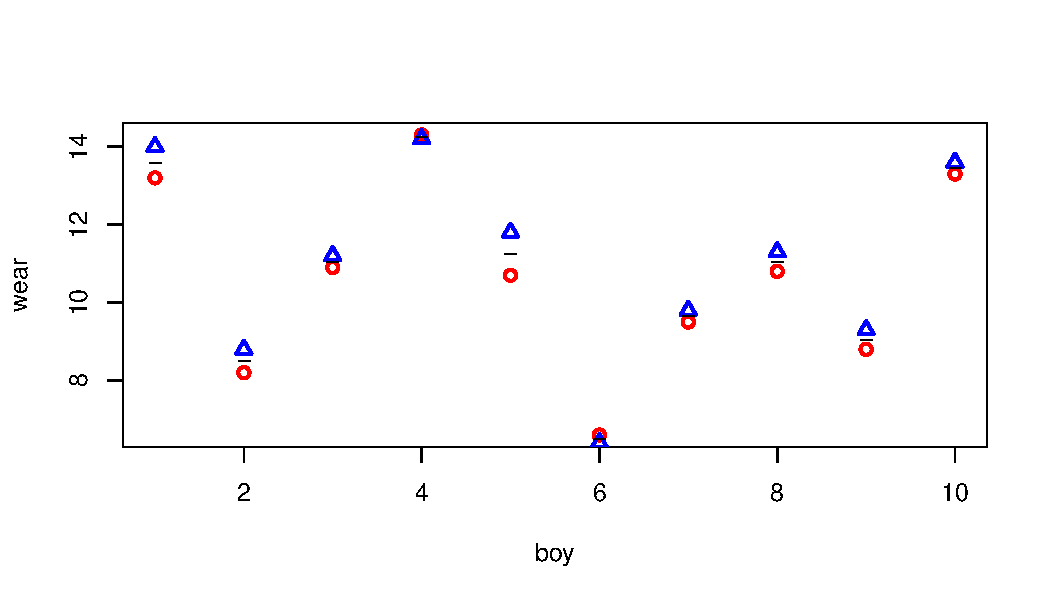
\includegraphics[width=\maxwidth]{figures/pbkrunnamed-chunk-5-1} 
\end{knitrout}


One option for testing the effect of materials is to make a paired
$t$--test. The following forms are equivalent:

\begin{knitrout}
\definecolor{shadecolor}{rgb}{0.969, 0.969, 0.969}\color{fgcolor}\begin{kframe}
\begin{alltt}
\hlstd{r1} \hlkwb{<-} \hlkwd{t.test}\hlstd{(shoes}\hlopt{$}\hlstd{A, shoes}\hlopt{$}\hlstd{B,} \hlkwc{paired}\hlstd{=T)}
\hlstd{r2} \hlkwb{<-} \hlkwd{t.test}\hlstd{(shoes}\hlopt{$}\hlstd{A} \hlopt{-} \hlstd{shoes}\hlopt{$}\hlstd{B)}
\hlstd{r1}
\end{alltt}
\begin{verbatim}
## 
## 	Paired t-test
## 
## data:  shoes$A and shoes$B
## t = -3.3489, df = 9, p-value = 0.008539
## alternative hypothesis: true mean difference is not equal to 0
## 95 percent confidence interval:
##  -0.6869539 -0.1330461
## sample estimates:
## mean difference 
##           -0.41
\end{verbatim}
\end{kframe}
\end{knitrout}


To work with data in a mixed model setting we create a dataframe, and
for later use we also create an imbalanced version of data:

\begin{knitrout}
\definecolor{shadecolor}{rgb}{0.969, 0.969, 0.969}\color{fgcolor}\begin{kframe}
\begin{alltt}
\hlstd{boy} \hlkwb{<-} \hlkwd{rep}\hlstd{(}\hlnum{1}\hlopt{:}\hlnum{10}\hlstd{,} \hlnum{2}\hlstd{)}
\hlstd{boyf}\hlkwb{<-} \hlkwd{factor}\hlstd{(letters[boy])}
\hlstd{mat} \hlkwb{<-} \hlkwd{factor}\hlstd{(}\hlkwd{c}\hlstd{(}\hlkwd{rep}\hlstd{(}\hlstr{"A"}\hlstd{,} \hlnum{10}\hlstd{),} \hlkwd{rep}\hlstd{(}\hlstr{"B"}\hlstd{,} \hlnum{10}\hlstd{)))}
\hlcom{## Balanced data:}
\hlstd{shoe.b} \hlkwb{<-} \hlkwd{data.frame}\hlstd{(}\hlkwc{wear}\hlstd{=}\hlkwd{unlist}\hlstd{(shoes),} \hlkwc{boy}\hlstd{=boy,} \hlkwc{boyf}\hlstd{=boyf,} \hlkwc{mat}\hlstd{=mat)}
\hlkwd{head}\hlstd{(shoe.b)}
\end{alltt}
\begin{verbatim}
##    wear boy boyf mat
## A1 13.2   1    a   A
## A2  8.2   2    b   A
## A3 10.9   3    c   A
## A4 14.3   4    d   A
## A5 10.7   5    e   A
## A6  6.6   6    f   A
\end{verbatim}
\begin{alltt}
\hlcom{## Imbalanced data; delete (boy=1, mat=1) and (boy=2, mat=b)}
\hlstd{shoe.i} \hlkwb{<-}  \hlstd{shoe.b[}\hlopt{-}\hlkwd{c}\hlstd{(}\hlnum{1}\hlstd{,} \hlnum{12}\hlstd{),]}
\end{alltt}
\end{kframe}
\end{knitrout}

We fit models to the two datasets:

\begin{knitrout}
\definecolor{shadecolor}{rgb}{0.969, 0.969, 0.969}\color{fgcolor}\begin{kframe}
\begin{alltt}
\hlstd{lmm1.b}  \hlkwb{<-} \hlkwd{lmer}\hlstd{( wear} \hlopt{~} \hlstd{mat} \hlopt{+} \hlstd{(}\hlnum{1}\hlopt{|}\hlstd{boyf),} \hlkwc{data}\hlstd{=shoe.b)}
\hlstd{lmm0.b}  \hlkwb{<-} \hlkwd{update}\hlstd{(lmm1.b, .}\hlopt{~}\hlstd{.} \hlopt{-} \hlstd{mat)}
\hlstd{lmm1.i}  \hlkwb{<-} \hlkwd{lmer}\hlstd{(wear} \hlopt{~} \hlstd{mat} \hlopt{+} \hlstd{(}\hlnum{1}\hlopt{|}\hlstd{boyf),} \hlkwc{data}\hlstd{=shoe.i)}
\hlstd{lmm0.i}  \hlkwb{<-} \hlkwd{update}\hlstd{(lmm1.i, .}\hlopt{~}\hlstd{.} \hlopt{-} \hlstd{mat)}
\end{alltt}
\end{kframe}
\end{knitrout}

The asymptotic likelihood ratio test shows stronger significance than
the $t$--test:

\begin{knitrout}
\definecolor{shadecolor}{rgb}{0.969, 0.969, 0.969}\color{fgcolor}\begin{kframe}
\begin{alltt}
\hlkwd{anova}\hlstd{(lmm1.b, lmm0.b,} \hlkwc{test}\hlstd{=}\hlstr{"Chisq"}\hlstd{)} \hlcom{## Balanced data}
\end{alltt}


{\ttfamily\noindent\itshape\color{messagecolor}{\#\# refitting model(s) with ML (instead of REML)}}\begin{verbatim}
## Data: shoe.b
## Models:
## lmm0.b: wear ~ (1 | boyf)
## lmm1.b: wear ~ mat + (1 | boyf)
##        npar    AIC    BIC  logLik deviance Chisq Df Pr(>Chisq)   
## lmm0.b    3 67.909 70.896 -30.955   61.909                       
## lmm1.b    4 61.817 65.800 -26.909   53.817 8.092  1   0.004446 **
## ---
## Signif. codes:  0 '***' 0.001 '**' 0.01 '*' 0.05 '.' 0.1 ' ' 1
\end{verbatim}
\begin{alltt}
\hlkwd{anova}\hlstd{(lmm1.i, lmm0.i,} \hlkwc{test}\hlstd{=}\hlstr{"Chisq"}\hlstd{)} \hlcom{## Imbalanced data}
\end{alltt}


{\ttfamily\noindent\itshape\color{messagecolor}{\#\# refitting model(s) with ML (instead of REML)}}\begin{verbatim}
## Data: shoe.i
## Models:
## lmm0.i: wear ~ (1 | boyf)
## lmm1.i: wear ~ mat + (1 | boyf)
##        npar    AIC    BIC  logLik deviance Chisq Df Pr(>Chisq)  
## lmm0.i    3 63.869 66.540 -28.934   57.869                      
## lmm1.i    4 60.777 64.339 -26.389   52.777 5.092  1    0.02404 *
## ---
## Signif. codes:  0 '***' 0.001 '**' 0.01 '*' 0.05 '.' 0.1 ' ' 1
\end{verbatim}
\end{kframe}
\end{knitrout}

\section{Kenward--Roger approach}
\label{sec:kenw-roger-appr}

The Kenward--Roger approximation is exact in certain balanced designs in the
sense that the approximation produces the same result as the paired $t$--test.

\begin{knitrout}
\definecolor{shadecolor}{rgb}{0.969, 0.969, 0.969}\color{fgcolor}\begin{kframe}
\begin{alltt}
\hlstd{kr.b} \hlkwb{<-} \hlkwd{KRmodcomp}\hlstd{(lmm1.b, lmm0.b)}
\hlstd{kr.b}
\end{alltt}
\begin{verbatim}
## large : wear ~ mat + (1 | boyf)
## small : wear ~ (1 | boyf)
##         stat    ndf    ddf F.scaling  p.value   
## Ftest 11.215  1.000  9.000         1 0.008539 **
## ---
## Signif. codes:  0 '***' 0.001 '**' 0.01 '*' 0.05 '.' 0.1 ' ' 1
\end{verbatim}
\end{kframe}
\end{knitrout}

\begin{knitrout}
\definecolor{shadecolor}{rgb}{0.969, 0.969, 0.969}\color{fgcolor}\begin{kframe}
\begin{alltt}
\hlkwd{summary}\hlstd{(kr.b)}
\end{alltt}
\begin{verbatim}
## F-test with Kenward-Roger approximation; time: 0.02 sec
## large : wear ~ mat + (1 | boyf)
## small : wear ~ (1 | boyf)
##          stat    ndf    ddf F.scaling  p.value   
## Ftest  11.215  1.000  9.000         1 0.008539 **
## FtestU 11.215  1.000  9.000           0.008539 **
## ---
## Signif. codes:  0 '***' 0.001 '**' 0.01 '*' 0.05 '.' 0.1 ' ' 1
\end{verbatim}
\end{kframe}
\end{knitrout}


For the imbalanced data we get
\begin{knitrout}
\definecolor{shadecolor}{rgb}{0.969, 0.969, 0.969}\color{fgcolor}\begin{kframe}
\begin{alltt}
\hlstd{kr.i} \hlkwb{<-} \hlkwd{KRmodcomp}\hlstd{(lmm1.i, lmm0.i)}
\hlstd{kr.i}
\end{alltt}
\begin{verbatim}
## large : wear ~ mat + (1 | boyf)
## small : wear ~ (1 | boyf)
##         stat    ndf    ddf F.scaling p.value  
## Ftest 5.9893 1.0000 7.0219         1 0.04418 *
## ---
## Signif. codes:  0 '***' 0.001 '**' 0.01 '*' 0.05 '.' 0.1 ' ' 1
\end{verbatim}
\end{kframe}
\end{knitrout}


Estimated degrees of freedom can be found with

\begin{knitrout}
\definecolor{shadecolor}{rgb}{0.969, 0.969, 0.969}\color{fgcolor}\begin{kframe}
\begin{alltt}
\hlkwd{c}\hlstd{(}\hlkwc{bal_ddf} \hlstd{=} \hlkwd{getKR}\hlstd{(kr.b,} \hlstr{"ddf"}\hlstd{),} \hlkwc{imbal_ddf} \hlstd{=} \hlkwd{getKR}\hlstd{(kr.i,} \hlstr{"ddf"}\hlstd{))}
\end{alltt}
\begin{verbatim}
##   bal_ddf imbal_ddf 
##  9.000000  7.021904
\end{verbatim}
\end{kframe}
\end{knitrout}


Notice that the Kenward-Roger approximation gives results  similar to but not identical to the paired
$t$--test when the two boys are removed:

\begin{knitrout}
\definecolor{shadecolor}{rgb}{0.969, 0.969, 0.969}\color{fgcolor}\begin{kframe}
\begin{alltt}
\hlstd{shoes2} \hlkwb{<-} \hlkwd{list}\hlstd{(}\hlkwc{A}\hlstd{=shoes}\hlopt{$}\hlstd{A[}\hlopt{-}\hlstd{(}\hlnum{1}\hlopt{:}\hlnum{2}\hlstd{)],} \hlkwc{B}\hlstd{=shoes}\hlopt{$}\hlstd{B[}\hlopt{-}\hlstd{(}\hlnum{1}\hlopt{:}\hlnum{2}\hlstd{)])}
\hlkwd{t.test}\hlstd{(shoes2}\hlopt{$}\hlstd{A, shoes2}\hlopt{$}\hlstd{B,} \hlkwc{paired}\hlstd{=T)}
\end{alltt}
\begin{verbatim}
## 
## 	Paired t-test
## 
## data:  shoes2$A and shoes2$B
## t = -2.3878, df = 7, p-value = 0.04832
## alternative hypothesis: true mean difference is not equal to 0
## 95 percent confidence interval:
##  -0.671721705 -0.003278295
## sample estimates:
## mean difference 
##         -0.3375
\end{verbatim}
\end{kframe}
\end{knitrout}


\section{Satterthwaite approach}
\label{sec:satterthwaite}

The Satterthwaite approximation is exact in certain balanced designs in the
sense that the approximation produces the same result as the paired $t$--test.

\begin{knitrout}
\definecolor{shadecolor}{rgb}{0.969, 0.969, 0.969}\color{fgcolor}\begin{kframe}
\begin{alltt}
\hlstd{sat.b} \hlkwb{<-} \hlkwd{SATmodcomp}\hlstd{(lmm1.b, lmm0.b)}
\hlstd{sat.b}
\end{alltt}
\begin{verbatim}
## large : wear ~ mat + (1 | boyf)
## small (restriction matrix) : 
##      
##  0 -1
##      statistic    ndf ddf  p.value   
## [1,]    11.215  1.000   9 0.008539 **
## ---
## Signif. codes:  0 '***' 0.001 '**' 0.01 '*' 0.05 '.' 0.1 ' ' 1
\end{verbatim}
\end{kframe}
\end{knitrout}

\begin{knitrout}
\definecolor{shadecolor}{rgb}{0.969, 0.969, 0.969}\color{fgcolor}\begin{kframe}
\begin{alltt}
\hlstd{sat.i} \hlkwb{<-} \hlkwd{SATmodcomp}\hlstd{(lmm1.i, lmm0.i)}
\hlstd{sat.i}
\end{alltt}
\begin{verbatim}
## large : wear ~ mat + (1 | boyf)
## small (restriction matrix) : 
##      
##  0 -1
##      statistic    ndf    ddf p.value  
## [1,]    5.9987 1.0000 7.0109  0.0441 *
## ---
## Signif. codes:  0 '***' 0.001 '**' 0.01 '*' 0.05 '.' 0.1 ' ' 1
\end{verbatim}
\end{kframe}
\end{knitrout}

Estimated degrees of freedom can be found with

\begin{knitrout}
\definecolor{shadecolor}{rgb}{0.969, 0.969, 0.969}\color{fgcolor}\begin{kframe}
\begin{alltt}
\hlkwd{c}\hlstd{(}\hlkwc{bal_ddf} \hlstd{=} \hlkwd{getSAT}\hlstd{(sat.b,} \hlstr{"ddf"}\hlstd{),} \hlkwc{imbal_ddf} \hlstd{=} \hlkwd{getSAT}\hlstd{(sat.i,} \hlstr{"ddf"}\hlstd{))}
\end{alltt}
\begin{verbatim}
##   bal_ddf imbal_ddf 
##  9.000000  7.010863
\end{verbatim}
\end{kframe}
\end{knitrout}


\section{Parametric bootstrap}
\label{sec:parametric-bootstrap}

Parametric bootstrap provides an alternative but many simulations are
often needed to provide credible results (also many more than shown
here; in this connection it can be useful to exploit that computings
can be made en parallel, see the documentation):

\begin{knitrout}
\definecolor{shadecolor}{rgb}{0.969, 0.969, 0.969}\color{fgcolor}\begin{kframe}
\begin{alltt}
\hlstd{pb.b} \hlkwb{<-} \hlkwd{PBmodcomp}\hlstd{(lmm1.b, lmm0.b,} \hlkwc{nsim}\hlstd{=}\hlnum{500}\hlstd{,} \hlkwc{cl}\hlstd{=}\hlnum{2}\hlstd{)}
\hlstd{pb.b}
\end{alltt}
\begin{verbatim}
## Bootstrap test; time: 3.08 sec; samples: 500; extremes: 6;
## large : wear ~ mat + (1 | boyf)
## wear ~ (1 | boyf)
##         stat df  p.value   
## LRT    8.092  1 0.004446 **
## PBtest 8.092    0.013972 * 
## ---
## Signif. codes:  0 '***' 0.001 '**' 0.01 '*' 0.05 '.' 0.1 ' ' 1
\end{verbatim}
\end{kframe}
\end{knitrout}

\begin{knitrout}
\definecolor{shadecolor}{rgb}{0.969, 0.969, 0.969}\color{fgcolor}\begin{kframe}
\begin{alltt}
\hlkwd{summary}\hlstd{(pb.b)}
\end{alltt}
\begin{verbatim}
## Bootstrap test; time: 3.08 sec; samples: 500; extremes: 6;
## large : wear ~ mat + (1 | boyf)
## wear ~ (1 | boyf)
##            stat     df    ddf  p.value   
## LRT      8.0920 1.0000        0.004446 **
## PBtest   8.0920               0.013972 * 
## Gamma    8.0920               0.011344 * 
## Bartlett 6.6977 1.0000        0.009654 **
## F        8.0920 1.0000 11.607 0.015204 * 
## ---
## Signif. codes:  0 '***' 0.001 '**' 0.01 '*' 0.05 '.' 0.1 ' ' 1
\end{verbatim}
\end{kframe}
\end{knitrout}


For the imbalanced data, the result is similar to the result from the
paired $t$ test.

\begin{knitrout}
\definecolor{shadecolor}{rgb}{0.969, 0.969, 0.969}\color{fgcolor}\begin{kframe}
\begin{alltt}
\hlstd{pb.i} \hlkwb{<-} \hlkwd{PBmodcomp}\hlstd{(lmm1.i, lmm0.i,} \hlkwc{nsim}\hlstd{=}\hlnum{500}\hlstd{,} \hlkwc{cl}\hlstd{=}\hlnum{2}\hlstd{)}
\hlstd{pb.i}
\end{alltt}
\begin{verbatim}
## Bootstrap test; time: 3.25 sec; samples: 500; extremes: 19;
## large : wear ~ mat + (1 | boyf)
## wear ~ (1 | boyf)
##         stat df p.value  
## LRT    5.092  1 0.02404 *
## PBtest 5.092    0.03992 *
## ---
## Signif. codes:  0 '***' 0.001 '**' 0.01 '*' 0.05 '.' 0.1 ' ' 1
\end{verbatim}
\end{kframe}
\end{knitrout}

\begin{knitrout}
\definecolor{shadecolor}{rgb}{0.969, 0.969, 0.969}\color{fgcolor}\begin{kframe}
\begin{alltt}
\hlkwd{summary}\hlstd{(pb.i)}
\end{alltt}
\begin{verbatim}
## Bootstrap test; time: 3.25 sec; samples: 500; extremes: 19;
## large : wear ~ mat + (1 | boyf)
## wear ~ (1 | boyf)
##            stat     df    ddf p.value  
## LRT      5.0920 1.0000        0.02404 *
## PBtest   5.0920               0.03992 *
## Gamma    5.0920               0.04148 *
## Bartlett 4.3063 1.0000        0.03797 *
## F        5.0920 1.0000 12.962 0.04195 *
## ---
## Signif. codes:  0 '***' 0.001 '**' 0.01 '*' 0.05 '.' 0.1 ' ' 1
\end{verbatim}
\end{kframe}
\end{knitrout}


\appendix

\section{Matrices for random effects}
\label{sec:matr-rand-effects}

The matrices involved in the random effects can be obtained with

\begin{knitrout}
\definecolor{shadecolor}{rgb}{0.969, 0.969, 0.969}\color{fgcolor}\begin{kframe}
\begin{alltt}
\hlstd{shoe3} \hlkwb{<-} \hlkwd{subset}\hlstd{(shoe.b, boy}\hlopt{<=}\hlnum{5}\hlstd{)}
\hlstd{shoe3} \hlkwb{<-} \hlstd{shoe3[}\hlkwd{order}\hlstd{(shoe3}\hlopt{$}\hlstd{boy), ]}
\hlstd{lmm1}  \hlkwb{<-} \hlkwd{lmer}\hlstd{( wear} \hlopt{~} \hlstd{mat} \hlopt{+} \hlstd{(}\hlnum{1}\hlopt{|}\hlstd{boyf),} \hlkwc{data}\hlstd{=shoe3 )}
\hlkwd{str}\hlstd{( SG} \hlkwb{<-} \hlkwd{get_SigmaG}\hlstd{( lmm1 ),} \hlkwc{max}\hlstd{=}\hlnum{2}\hlstd{)}
\end{alltt}
\begin{verbatim}
## List of 3
##  $ Sigma   :Formal class 'dgCMatrix' [package "Matrix"] with 6 slots
##  $ G       :List of 2
##   ..$ :Formal class 'dgCMatrix' [package "Matrix"] with 6 slots
##   ..$ :Formal class 'dgCMatrix' [package "Matrix"] with 6 slots
##  $ n.ggamma: int 2
\end{verbatim}
\end{kframe}
\end{knitrout}

\begin{knitrout}
\definecolor{shadecolor}{rgb}{0.969, 0.969, 0.969}\color{fgcolor}\begin{kframe}
\begin{alltt}
\hlkwd{round}\hlstd{( SG}\hlopt{$}\hlstd{Sigma}\hlopt{*}\hlnum{10} \hlstd{)}
\end{alltt}
\begin{verbatim}
## 10 x 10 sparse Matrix of class "dgCMatrix"
\end{verbatim}


{\ttfamily\noindent\itshape\color{messagecolor}{\#\# \ \ [[ suppressing 10 column names 'A1', 'B1', 'A2' ... ]]}}\begin{verbatim}
##                                 
## A1 53 52  .  .  .  .  .  .  .  .
## B1 52 53  .  .  .  .  .  .  .  .
## A2  .  . 53 52  .  .  .  .  .  .
## B2  .  . 52 53  .  .  .  .  .  .
## A3  .  .  .  . 53 52  .  .  .  .
## B3  .  .  .  . 52 53  .  .  .  .
## A4  .  .  .  .  .  . 53 52  .  .
## B4  .  .  .  .  .  . 52 53  .  .
## A5  .  .  .  .  .  .  .  . 53 52
## B5  .  .  .  .  .  .  .  . 52 53
\end{verbatim}
\end{kframe}
\end{knitrout}

\begin{knitrout}
\definecolor{shadecolor}{rgb}{0.969, 0.969, 0.969}\color{fgcolor}\begin{kframe}
\begin{alltt}
\hlstd{SG}\hlopt{$}\hlstd{G}
\end{alltt}
\begin{verbatim}
## [[1]]
## 10 x 10 sparse Matrix of class "dgCMatrix"
\end{verbatim}


{\ttfamily\noindent\itshape\color{messagecolor}{\#\# \ \ [[ suppressing 10 column names 'A1', 'B1', 'A2' ... ]]}}\begin{verbatim}
##                       
## A1 1 1 . . . . . . . .
## B1 1 1 . . . . . . . .
## A2 . . 1 1 . . . . . .
## B2 . . 1 1 . . . . . .
## A3 . . . . 1 1 . . . .
## B3 . . . . 1 1 . . . .
## A4 . . . . . . 1 1 . .
## B4 . . . . . . 1 1 . .
## A5 . . . . . . . . 1 1
## B5 . . . . . . . . 1 1
## 
## [[2]]
## 10 x 10 sparse Matrix of class "dgCMatrix"
##                          
##  [1,] 1 . . . . . . . . .
##  [2,] . 1 . . . . . . . .
##  [3,] . . 1 . . . . . . .
##  [4,] . . . 1 . . . . . .
##  [5,] . . . . 1 . . . . .
##  [6,] . . . . . 1 . . . .
##  [7,] . . . . . . 1 . . .
##  [8,] . . . . . . . 1 . .
##  [9,] . . . . . . . . 1 .
## [10,] . . . . . . . . . 1
\end{verbatim}
\end{kframe}
\end{knitrout}

\end{document}

